\section*{Đề thi thử THPTQG Sở GD\&ĐT 25--26, Thành phố Đà Nẵng}

\caulc
\Opensolutionfile{ans}[ans/ans-39-26-2-DaNang-SoGD-L1-LC]
%%==========Câu 1
\begin{ex}%[39-26-2-DaNang-SoGD-L1]%[Tuấn Anh,26-2-DuAnDeTHPT2025-2026]%[1D6N4-2]
	Nghiệm của phương trình $\log(4x-8)=2$ là
	\choice
	{$x=\dfrac{5}{2}$}
	{$x=\dfrac{\mathrm{e}^2+8}{4}$}
	{\True $x=27$}
	{$x=256$}
	\loigiai{
		Điều kiện xác định của phương trình là $4x-8>0 \Leftrightarrow x>2$.\\
		Ta có
		\begin{eqnarray*}
			\log(4x-8)&=&2\\
			4x-8&=&10^2\\
			x&=&27\,\text{(thỏa mãn điều kiện)}.
		\end{eqnarray*}
		Vậy nghiệm của phương trình là $x=27$.
	}
\end{ex}

%%==========Câu 2
\begin{ex}%[39-26-2-DaNang-SoGD-L1]%[Tuấn Anh,26-2-DuAnDeTHPT2025-2026]%[2D4N1-2]
	Nguyên hàm của hàm số $f(x)=\dfrac{x+1}{x}$ trên khoảng $(0;+\infty)$ là
	\choice
	{$-\dfrac{1}{x^2}+C$}
	{$\ln x+C$}
	{$\dfrac{1}{x^2}+C$}
	{\True $x+\ln x+C$}
	\loigiai{
		Vì $f(x)=\dfrac{x+1}{x}=1+\dfrac{1}{x}$ nên $\displaystyle\int \dfrac{x+1}{x}\mathrm{\,d}x
		=\int \left(1+\dfrac{1}{x}\right)\mathrm{\,d}x
		=x+\ln |x|+C$.\\
		Vì $x\in(0;+\infty)$ nên $|x|=x$.\\
		Vậy nguyên hàm của hàm số là $x+\ln x+C$.
	}
\end{ex}

%%==========Câu 3
\begin{ex}%[39-26-2-DaNang-SoGD-L1]%[Tuấn Anh,26-2-DuAnDeTHPT2025-2026]%[1D6N4-3]
	Tập nghiệm của bất phương trình $0{,}5^x\leq 4$ là
	\choice
	{\True $[-2;+\infty)$}
	{$\left(-\infty;-\dfrac{1}{2}\right]$}
	{$(-\infty;-2]$}
	{$\left[-\dfrac{1}{2};+\infty\right)$}
	\loigiai{
		Ta có
		\begin{eqnarray*}
			0{,}5^x &\leq& 4\\
			\left(\dfrac{1}{2}\right)^x&\leq& 2^2\\
			2^{-x}&\leq& 2^2\\
			-x&\leq& 2\\
			x&\geq& -2.
		\end{eqnarray*}
		Vậy tập nghiệm của bất phương trình là $[-2;+\infty)$.
	}
\end{ex}

%%==========Câu 4
\begin{ex}%[39-26-2-DaNang-SoGD-L1]%[Tuấn Anh,26-2-DuAnDeTHPT2025-2026]%[1D1N5-3]
	Tập nghiệm của phương trình $\tan x=1$ là
	\choice
	{$S=\left\{-\dfrac{\pi}{4}+k\pi, k\in\mathbb{Z}\right\}$}
	{$S=\left\{-\dfrac{\pi}{4}+k2\pi, k\in\mathbb{Z}\right\}$}
	{\True $S=\left\{\dfrac{\pi}{4}+k\pi, k\in\mathbb{Z}\right\}$}
	{$S=\left\{\dfrac{\pi}{4}+k2\pi, k\in\mathbb{Z}\right\}$}
	\loigiai{
		Ta có
		\begin{eqnarray*}
			\tan x&=&1\\
			\tan x&=&\tan \dfrac{\pi}{4}\\
			x&=&\dfrac{\pi}{4}+k\pi,\ k\in\mathbb{Z}.
		\end{eqnarray*}
		Vậy tập nghiệm của phương trình là $S=\left\{\dfrac{\pi}{4}+k\pi, k\in\mathbb{Z}\right\}$.
	}
\end{ex}

%%==========Câu 5
\begin{ex}%[39-26-2-DaNang-SoGD-L1]%[Tuấn Anh,26-2-DuAnDeTHPT2025-2026]%[2H2N1-2]
	\immini[thm]{Cho hình chóp $S.ABC$ như hình bên. Tìm mệnh đề đúng.
		\choice
		{$\overrightarrow{AB}+\overrightarrow{BC}-\overrightarrow{AS}=\overrightarrow{AS}$}
		{$\overrightarrow{AB}+\overrightarrow{BC}-\overrightarrow{AS}=\overrightarrow{SA}$}
		{$\overrightarrow{AB}+\overrightarrow{BC}-\overrightarrow{AS}=\overrightarrow{CS}$}
		{\True $\overrightarrow{AB}+\overrightarrow{BC}-\overrightarrow{AS}=\overrightarrow{SC}$}
	}
	{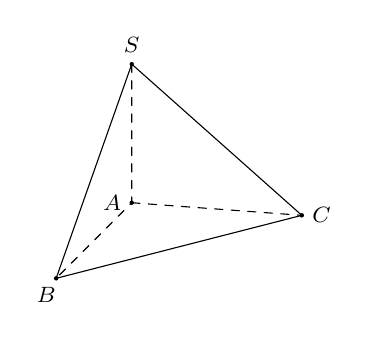
\begin{tikzpicture}[scale=0.8, font=\footnotesize, line join=round, line cap=round, >=stealth]
		\coordinate (A) at (0,0);
		\coordinate (B) at (-1.2,-1.2);
		\coordinate (C) at (2.7,-0.2);
		\coordinate (S) at (0,2.2);
		\draw (S)--(B)--(C)--(S);
		\draw[dashed] (S)--(A)--(B) (A)--(C);
		\fill (A) circle(1pt) node[shift=(180:0.25)]{$A$}
		(B) circle(1pt) node[shift=(-120:0.25)]{$B$}
		(C) circle(1pt) node[shift=(0:0.25)]{$C$}
		(S) circle(1pt) node[shift=(90:0.25)]{$S$};
	\end{tikzpicture}}
	\loigiai{
		Ta có
		$\overrightarrow{AB}+\overrightarrow{BC}-\overrightarrow{AS}
		=\overrightarrow{AC}+\overrightarrow{SA}
		=\overrightarrow{SC}$.
	}
\end{ex}

%%==========Câu 6
\begin{ex}%[39-26-2-DaNang-SoGD-L1]%[Tuấn Anh,26-2-DuAnDeTHPT2025-2026]%[1H8H7-3]
	Cho hình chóp $S.ABCD$ có đáy $ABCD$ là hình thoi và $SA$ vuông góc với mặt phẳng $(ABCD)$. Biết $SA=3$, $AC=4$, $BD=5$. Thể tích khối chóp $S.ABCD$ bằng
	\choice
	{\True $10$}
	{$20$}
	{$30$}
	{$60$}
	\loigiai{
		\begin{center}
			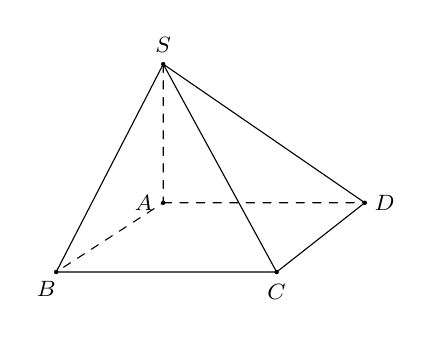
\begin{tikzpicture}[scale=0.8, font=\footnotesize, line join=round, line cap=round, >=stealth]
				\coordinate (A) at (0,0);
				\coordinate (B) at (-1.7,-1.1);
				\coordinate (C) at (1.8,-1.1);
				\coordinate (D) at (3.2,0);
				\coordinate (S) at (0,2.2);
				\draw (S)--(B)--(C)--(D)--(S)--(C);
				\draw[dashed] (S)--(A)--(B) (A)--(D);
				\fill (A) circle(1pt) node[shift=(180:0.25)]{$A$}
				(B) circle(1pt) node[shift=(-120:0.25)]{$B$}
				(C) circle(1pt) node[shift=(-90:0.25)]{$C$}
				(D) circle(1pt) node[shift=(0:0.25)]{$D$}
				(S) circle(1pt) node[shift=(90:0.25)]{$S$};
			\end{tikzpicture}
		\end{center}
		Đáy $ABCD$ là hình thoi có độ dài hai đường chéo $AC=4$ và $BD=5$.\\
		Diện tích đáy của hình chóp là $S_{ABCD}=\dfrac{1}{2}\cdot AC\cdot BD=\dfrac{1}{2}\cdot 4\cdot 5=10$.\\
		Chiều cao của hình chóp là $h=SA=3$ vì $SA\perp(ABCD)$.\\
		Thể tích khối chóp $S.ABCD$ là $V=\dfrac{1}{3}\cdot S_{ABCD}\cdot h=\dfrac{1}{3}\cdot 10\cdot 3=10$.
	}
\end{ex}

%%==========Câu 7
\begin{ex}%[39-26-2-DaNang-SoGD-L1]%[Tuấn Anh,26-2-DuAnDeTHPT2025-2026]%[2H5N2-2]
	Trong không gian $Oxyz$, đường thẳng $\dfrac{x}{3}=\dfrac{y+1}{-4}=\dfrac{z-2}{5}$ có một vectơ chỉ phương là
	\choice
	{$\overrightarrow{u}_3=(0;-1;2)$}
	{$\overrightarrow{u}_1=(3;4;5)$}
	{\True $\overrightarrow{u}_4=(3;-4;5)$}
	{$\overrightarrow{u}_2=(0;1;-2)$}
	\loigiai{
		Từ phương trình chính tắc $\dfrac{x}{3}=\dfrac{y+1}{-4}=\dfrac{z-2}{5}$.\\
		Suy ra đường thẳng có một vectơ chỉ phương là $\overrightarrow{u}=(3;-4;5)$.
	}
\end{ex}

%%==========Câu 8
\begin{ex}%[39-26-2-DaNang-SoGD-L1]%[Tuấn Anh,26-2-DuAnDeTHPT2025-2026]%[1D2N3-4]
	Cấp số nhân $(u_n)$ có số hạng đầu là $u_1=-2$ và công bội $q=3$ thì có số hạng $u_4$ bằng
	\choice
	{$7$}
	{$-18$}
	{$81$}
	{\True $-54$}
	\loigiai{
		Cấp số nhân $(u_n)$ có số hạng đầu là $u_1=-2$ và công bội $q=3$.\\
		Ta có $u_4=u_1\cdot q^3=-2\cdot 3^3=-54$.
	}
\end{ex}

%%==========Câu 9
\begin{ex}%[39-26-2-DaNang-SoGD-L1]%[Tuấn Anh,26-2-DuAnDeTHPT2025-2026]%[1D5H2-2]
	Theo một báo cáo của Common Sense Media, thời gian sử dụng thiết bị số của thanh thiếu niên có thể liên quan đến hiện tượng \lq\lq Brain rot\rq\rq\ suy giảm khả năng tập trung do sử dụng quá nhiều nội dung số, như video ngắn, đang ngày càng phổ biến ở học sinh. Một khảo sát $100$ học sinh lớp $12$ cho kết quả như sau
	\begin{center}
		\begin{tabular}{|c|c|c|c|c|c|}
			\hline
			\begin{tabular}{c}
				Thời gian\\(giờ)
			\end{tabular} & $[0;2)$ & $[2;4)$ & $[4;6)$ & $[6;8)$ & $[8;10)$ \\
			\hline
			Số học sinh & $10$ & $20$ & $30$ & $25$ & $15$ \\
			\hline
		\end{tabular}
	\end{center}
	Nhóm chứa trung vị của mẫu số liệu trên là
	\choice
	{$[2;4)$}
	{$[8;10)$}
	{$[6;8)$}
	{\True $[4;6)$}
	\loigiai{
		Ta có $\dfrac{n}{2}=\dfrac{100}{2}=50$.\\
		Bảng tần số tích lũy cho thấy giá trị thứ $50$ thuộc nhóm $[4;6)$.\\
		Suy ra nhóm chứa trung vị của mẫu số liệu trên là $[4;6)$.
	}
\end{ex}

%%==========Câu 10
\begin{ex}%[39-26-2-DaNang-SoGD-L1]%[Tuấn Anh,26-2-DuAnDeTHPT2025-2026]%[1H8N2-2]
	\immini[thm]{Cho hình hộp chữ nhật $ABCD.A'B'C'D'$ như hình bên. Mặt phẳng $(ABCD)$ vuông góc với đường thẳng
		\choice
		{$AB'$}
		{$B'D$}
		{$A'B'$}
		{\True $BB'$}
	}
	{
		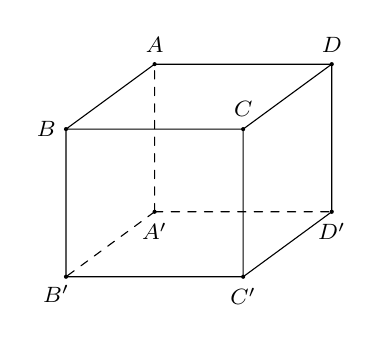
\begin{tikzpicture}[scale=0.75, font=\footnotesize, line join=round, line cap=round, >=stealth]
			\coordinate (B') at (0,0);
			\coordinate (C') at (3,0);
			\coordinate (D') at (4.5,1.1);
			\coordinate (A') at (1.5,1.1);
			\coordinate (B) at (0,2.5);
			\coordinate (C) at (3,2.5);
			\coordinate (D) at (4.5,3.6);
			\coordinate (A) at (1.5,3.6);
			\draw (B')--(C')--(D')--(D)--(A)--(B)--(B') (B)--(C)--(D) (C)--(C');
			\draw (A)--(D);
			\draw[dashed] (A')--(A) (A')--(B') (A')--(D');
			\fill (A) circle(1pt) node[shift=(90:0.25)]{$A$}
			(B) circle(1pt) node[shift=(180:0.25)]{$B$}
			(C) circle(1pt) node[shift=(90:0.25)]{$C$}
			(D) circle(1pt) node[shift=(90:0.25)]{$D$}
			(A') circle(1pt) node[shift=(-90:0.25)]{$A'$}
			(B') circle(1pt) node[shift=(-120:0.25)]{$B'$}
			(C') circle(1pt) node[shift=(-90:0.25)]{$C'$}
			(D') circle(1pt) node[shift=(-90:0.25)]{$D'$};
		\end{tikzpicture}
	}
	\loigiai{
		Vì $ABCD.A'B'C'D'$ là hình hộp chữ nhật nên các cạnh bên $AA'$, $BB'$, $CC'$, $DD'$ cùng vuông góc với mặt phẳng $(ABCD)$.\\
		Do đó $(ABCD)\perp BB'$.
	}
\end{ex}

%%==========Câu 11
\begin{ex}%[39-26-2-DaNang-SoGD-L1]%[Tuấn Anh,26-2-DuAnDeTHPT2025-2026]%[2H5H1-3]
	Trong không gian $Oxyz$, cho điểm $M(0;-1;0)$ và điểm $N(5;0;-2)$. Mặt phẳng đi qua điểm $M$ và vuông góc với $MN$ có phương trình là
	\choice
	{$5x+y-2z-29=0$}
	{\True $5x+y-2z+1=0$}
	{$5x-y-2z-1=0$}
	{$5x+y-2z-1=0$}
	\loigiai{
		Mặt phẳng đi qua điểm $M$ và vuông góc với $MN$ nên mặt phẳng đi qua điểm $M(0;-1;0)$ và có một vectơ pháp tuyến là $\overrightarrow{MN}=(5;1;-2)$.
		Phương trình mặt phẳng là
		\[5(x-0)+(y+1)-2(z-0)=0\Leftrightarrow 5x+y-2z+1=0.\]
	}
\end{ex}

%%==========Câu 12
\begin{ex}%[39-26-2-DaNang-SoGD-L1]%[Tuấn Anh,26-2-DuAnDeTHPT2025-2026]%[2D1N4-1]
	Đồ thị hàm số $y=\dfrac{2x-1}{x+2}$ có tiệm cận ngang là
	\choice
	{\True $y=2$}
	{$y=-2$}
	{$y=-\dfrac{1}{2}$}
	{$y=\dfrac{1}{2}$}
	\loigiai{
		Ta có $\lim\limits_{x\to \pm\infty}\dfrac{2x-1}{x+2}=2$.\\
		Vậy đồ thị hàm số có tiệm cận ngang là $y=2$.
	}
\end{ex}

\Closesolutionfile{ans}


\cauds
\Opensolutionfile{ans}[ans/ans-39-26-2-DaNang-SoGD-L1-DS]
%%==========Câu 1
\begin{ex}%[39-26-2-DaNang-SoGD-L1]%[Tuấn Anh,26-2-DuAnDeTHPT2025-2026]%[2D6H2-3]
	Trong một buổi hội thảo chuyên đề về ứng dụng trí tuệ nhân tạo (AI) trong học tập, có $300$ học sinh khối $11$ và $200$ học sinh khối $12$ tham gia. Qua khảo sát thực tế, tỉ lệ học sinh khối $11$ có sử dụng hệ thống chatbot AI hỗ trợ học tập là $0{,}4$; trong khi tỉ lệ này ở khối $12$ là $0{,}7$. Ban tổ chức chọn ngẫu nhiên một học sinh tham gia hội thảo để phỏng vấn.
	\choiceTF
	{\True Xác suất để học sinh được chọn tham gia phỏng vấn thuộc khối $12$ là $0{,}4$}
	{\True Xác suất để chọn được một học sinh khối $11$ và em này sử dụng chatbot AI là $0{,}24$}
	{Xác suất để học sinh được chọn có sử dụng chatbot AI là $0{,}55$}
	{\True Giả sử học sinh được chọn phỏng vấn cho biết mình có sử dụng chatbot AI, xác suất học sinh đó thuộc khối $12$ là $\dfrac{7}{13}$}
	\loigiai{
		Tổng số học sinh là $300+200=500$.\\
		Gọi
		\begin{itemize}
			\item Biến cố $A\colon$\lq\lq Chọn một học sinh khối $11$\rq\rq, suy ra $P(A)=\dfrac{300}{500}=0{,}6$.
			\item Biến cố $\overline{A}\colon$\lq\lq Chọn một học sinh khối $12$\rq\rq, suy ra $P\big(\overline{A}\big)=\dfrac{200}{500}=0{,}4$.
			\item Biến cố $B\colon$\lq\lq Chọn được học sinh có sử dụng AI\rq\rq.
			\item Biến cố $\overline{B}\colon$\lq\lq Chọn được học sinh không sử dụng AI\rq\rq.
		\end{itemize}
		Theo đề bài, ta có $P(B\mid A)=0{,}4$; $P\big(\overline{B}\mid A\big)=0{,}6$; $P\big(B\mid\overline{A}\big)=0{,}7$ và $P\big(\overline{B}\mid\overline{A}\big)=0{,}3$.
		\begin{itemchoice}
			\itemch Xác suất để học sinh được chọn tham gia phỏng vấn thuộc khối $12$ là $P\big(\overline{A}\big)=0{,}4$.
			\itemch Xác suất để chọn được một học sinh khối $11$ và em này sử dụng chatbot AI là \[P(AB)=P(A)\cdot P(B\mid A)=0{,}6\cdot 0{,}4=0{,}24.\]
			\itemch Xác suất để học sinh được chọn có sử dụng chatbot AI là
			\begin{eqnarray*}
				P(B)&=&P(A)P\left(B\mid A\right)+P\big(\overline{A}\big)P\left(B\mid\overline{A}\right)\\
				&=&0{,}6\cdot 0{,}4+0{,}4\cdot 0{,}7\\
				&=&0{,}52.
			\end{eqnarray*}
			\itemch Giả sử học sinh được chọn phỏng vấn cho biết mình có sử dụng chatbot AI, xác suất học sinh đó thuộc khối $12$ là \begin{eqnarray*}
				P\left(\overline{A}\mid B\right)&=&\dfrac{P\big(\overline{A}\big)P\left(B\mid\overline{A}\right)}{P(B)}\\
				&=&\dfrac{0{,}4\cdot 0{,}7}{0{,}52}\\
				&=&\dfrac{7}{13}.
			\end{eqnarray*}
		\end{itemchoice}
	}
\end{ex}

%%==========Câu 2
\begin{ex}%[39-26-2-DaNang-SoGD-L1]%[Tuấn Anh,26-2-DuAnDeTHPT2025-2026]%[2H5V2-8]
	Bay Flycam trái phép là hành vi tiềm ẩn nguy cơ uy hiếp trực tiếp an toàn hàng không, lĩnh vực liên quan tới tính mạng của hàng trăm hành khách trên mỗi chuyến bay. Một cảng hàng không quốc tế thiết lập hệ thống rada giám sát được đặt tại gốc tọa độ $O(0;0;0)$ trong không gian $Oxyz$ (đơn vị: $1$ km, mặt phẳng $Oxy$ là mặt đất). Tại thời điểm $t=0$, radar phát hiện một flycam tại điểm $A(4;2;2)$ đang bay theo đường thẳng với vectơ vận tốc $\overrightarrow{v}_1=(-1;0;0)$ (đơn vị: km/phút). Cùng lúc đó, máy bay A$321$ đang chờ lệnh cất cánh tại điểm $B(0;-2;0)$, Nếu được cấp phép, quỹ đạo cất cánh dự kiến của máy bay là đường thẳng với vectơ vận tốc $\overrightarrow{v}_2=(0;4;3)$ (đơn vị: km/phút). Kiểm soát viên không lưu không được phép cấp lệnh cất cánh cho máy bay thương mại nếu hệ thống dự báo có bất kỳ thời điểm nào khoảng cách giữ hai máy bay và thể lạ nhỏ hơn $5$ km.
	\choiceTF
	{\True Khoảng cách từ vị trí ban đầu của máy bay đến Flycam tại thời điểm phát hiện lớn hơn $5$ km}
	{\True Phương trình đường thẳng mô tả quỹ đạo máy bay cất cánh là $\heva{&x=0\\ &y=-2+4t\\ &z=3t}$}
	{Tốc độ của Flycam là $1$ km/h và tốc độ cất cánh dự kiến của máy bay A$321$ là $300$ km/h}
	{\True Nếu máy bay A$321$ được phép cất cánh, khoảng cách ngắn nhất giữa nó với chiếc Flycam sẽ đạt được vào thời điểm $1$ phút kể từ lúc rời đường băng}
	\loigiai{
		\begin{itemchoice}
			\itemch Ta có $\overrightarrow{AB}=(-4;-4;-2)$.\\
			Suy ra khoảng cách từ vị trí ban đầu của máy bay đến Flycam tại thời điểm phát hiện là \[AB=\sqrt{(-4)^2+(-4)^2+(-2)^2}=6>5.\]
			\itemch Máy bay chở khách A$321$ đang chờ lệnh cất cánh tại điểm $B(0;-2;0)$ vectơ vận tốc là $\overrightarrow{v}_2=(0;4;3)$.\\
			Suy ra phương trình đường thẳng mô tả quỹ đạo máy bay cất cánh là
			$\heva{&x=0\\&y=-2+4t\\&z=3t.}$
			\itemch  Ta có
			\begin{itemize}
				\item $\left|\overrightarrow{v}_1\right|=\sqrt{(-1)^2}=1$ km/phút$=60$ km/h.
				\item $\left|\overrightarrow{v}_2\right|=\sqrt{4^2+3^2}=5$ km/phút$=300$ km/h.
			\end{itemize}
			Vậy tốc độ Flycam là $60$ km/h và tốc độ cất cánh dự kiến của máy bay A$321$ là $300$ km/h.\\
			\itemch Ta có phương trình đường thẳng mô tả
			\begin{itemize}
				\item Quỹ đạo máy bay cất cánh là $\Delta_1\colon\heva{&x=0\\&y=-2+4t\\&z=3t.}$
				\item Sự di chuyển của Flycam là $\Delta_2\colon\heva{&x=4-t\\&y=2\\&z=2.}$
			\end{itemize}
			Gọi $M$, $N$ lần lượt là vị trí của máy bay và Flycam tại thời điểm $t$ phút.\\
			Khi đó $M(0;-2+4t;3t)$, $N(4-t;2;2)\Rightarrow \overrightarrow{MN}=(4-t;4-4t;2-3t)$.\\
			Suy ra $MN^2=(4-t)^2+(4-4t)^2+(2-3t)^2=26t^2-52t+36$.\\
			Đặt $f(t)=26t^2-52t+36\Rightarrow f'(t)=52t-52$.\\
			Khi đó $f'(t)=0\Leftrightarrow t=1$.\\
			Bảng biến thiên
			\begin{center}
				
\begin{tikzpicture}
					\tkzTabInit[lgt=1.2,espcl=3]
					{$t$ /1.2, $f’(t)$ /1.2, $f(t)$ /2.5}
					{$-\infty$,$1$,$+\infty$}
					\tkzTabLine{,-,z,+,}
					\tkzTabVar{+/$+\infty$,-/$10$,+/$+\infty$}
				\end{tikzpicture}
			\end{center}
			Suy ra $MN_{\text{min}}=f(1)=10$.\\
			Vậy khoảng cách ngắn nhất giữa máy bay với chiếc Flycam sẽ đạt được vào thời điểm $1$ phút kể từ lúc rời đường băng.
		\end{itemchoice}
	}
\end{ex}

%%==========Câu 3
\begin{ex}%[39-26-2-DaNang-SoGD-L1]%[Tuấn Anh,26-2-DuAnDeTHPT2025-2026]%[2D1H4-1]
	Cho hàm số $f(x)=\dfrac{x^2-2x+3}{x-1}$.
	\choiceTF
	{\True Tiệm cận đứng của đồ thị hàm số đã cho là đường thẳng $x=1$}
	{Hàm số đã cho có đạo hàm $f'(x)=\dfrac{x^2-2x+2}{(x-1)^2},\forall x\neq 1$}
	{\True Hàm số $f(x)$ có hai điểm cực trị}
	{\True Hàm số $f(x)$ không có giá trị nhỏ nhất trên khoảng $(1;+\infty)$}
	\loigiai{
		\begin{itemchoice}
			\itemch Do $\lim\limits_{x\rightarrow1^+}f(x)=\lim\limits_{x\rightarrow1^+}\dfrac{x^2-2x+3}{x-1}=+\infty$.\\
			Nên đồ thị hàm số có tiệm cận đứng là đường thẳng $x=1$.
			\itemch Ta có
			\begin{eqnarray*}
				f'(x)&=&\dfrac{(2x-2)(x-1)-\left(x^2-2x+3\right)}{(x-1)^2}\\
				&=&\dfrac{2x^2-4x+2-x^2+2x-3}{(x-1)^2}\\
				&=&\dfrac{x^2-2x-1}{(x-1)^2},\,\forall x\neq 1.
			\end{eqnarray*}
			\itemch Do $f'(x)=0\Leftrightarrow\dfrac{x^2-2x-1}{(x-1)^2}=0\Leftrightarrow x^2-2x-1=0\Leftrightarrow\hoac{&x=1+\sqrt{2}\\&x=1-\sqrt{2}.}$\\
			Bảng biến thiên
			\begin{center}
				
\begin{tikzpicture}
					\tkzTabInit[lgt=1.2,espcl=3]
					{$x$ /1.2, $f’(x)$ /1.2, $f(x)$ /2.5}
					{$-\infty$,$1-\sqrt{2}$,$1$,$1+\sqrt{2}$,$+\infty$}
					\tkzTabLine{,+,z,-,d,-,z,+,}
					\tkzTabVar{-/$-\infty$,+/$-2\sqrt{2}$,-D+/$-\infty$/$+\infty$,-/$2\sqrt{2}$,+/$+\infty$}
				\end{tikzpicture}
			\end{center}
			Vậy hàm số $f(x)$ có hai điểm cực trị.
			\itemch Hàm số $f(x)$ đạt giá trị nhỏ nhất bằng $2\sqrt{2}$ tại $x=1+\sqrt{2}$ trên khoảng $(1;+\infty)$.
		\end{itemchoice}
	}
\end{ex}

%%==========Câu 4
\begin{ex}%[39-26-2-DaNang-SoGD-L1]%[Tuấn Anh,26-2-DuAnDeTHPT2025-2026]%[2D1H2-7]
	Trong công nghệ ô tô điện (EV), Hệ thống Quản lý Pin (BMS) của xe sẽ tự động điều chỉnh dòng	điện để bảo vệ tuổi thọ pin. Một trạm sạc DC siêu nhanh có công suất truyền vào pin $P(t)$ (kW) theo thời gian $t$ (giờ) kể từ lúc bắt đầu cắm sạc được tính bằng hàm số $P(t)=250\,\mathrm{e}^{-kt}$, với $k$ là một hằng số dương đặc trưng cho giới hạn tản nhiệt của dòng xe đó. Biết rằng, ngay tại thời điểm vừa cắm sạc, tốc độ sụt giảm công suất sạc là $625$ kW/giờ. Thực tế, BMS của xe sẽ tự động ngắt sạc (báo pin đầy) khi công suất sạc giảm xuống chỉ còn bằng $1\%$ so với công suất ban đầu.
	\choiceTF
	{\True Công suất sạc ban đầu ngay khi cắm sạc là $250$ kW}
	{Tốc độ thay đổi công suất tại thời điểm $t$ là $P'(t)=250\,k\mathrm{e}^{-kt}$}
	{\True Công suất sạc giảm dần theo thời gian và $k=2{,}5$}
	{\True Thời gian từ lúc bắt đầu sạc đến khi hệ thống tự ngắt kéo dài không quá $111$ phút (kết quả làm tròn đến hàng đơn vị)}
	\loigiai{
		\begin{itemchoice}
			\itemch Công suất sạc ban đầu ngay khi cắm sạc là $P(0)=250\,\mathrm{e}^{-k\cdot 0}=250$ (kW).
			\itemch Tốc độ thay đổi công suất tại thời điểm $t$ là $P'(t)=250\left(\mathrm{e}^{-kt}\right)'=-250\,k\mathrm{e}^{-kt}$.
			\itemch Tại thời điểm vừa cắm sạc, tốc độ sụt giảm công suất sạc là $625$ kW/giờ.\\
			Nên $P'(0)=-625\Leftrightarrow -250k=-625\Leftrightarrow k=2{,}5$.\\
			Vậy công suất sạc giảm dần theo thời gian và $k=2{,}5$.
			\itemch Thực tế, BMS của xe sẽ tự động ngắt sạc (báo pin đầy) khi công suất sạc giảm xuống chỉ còn bằng $1\%$ so với công suất ban đầu.\\
			Nên $250\cdot\mathrm{e}^{2{,}5t}=250\cdot0{,}01\Leftrightarrow\mathrm{e}^{-2{,}5t}=0{,}01\Leftrightarrow -2{,}5t=\ln\left(0{,}01\right)\Leftrightarrow t\approx 1{,}84$ (giờ).\\
			Vậy thời gian từ lúc bắt đầu cắm sạc đến khi hệ thống tự ngắt kéo dài không quá $t\approx111$ phút.
		\end{itemchoice}
	}
\end{ex}
\Closesolutionfile{ans}

\caukq
\Opensolutionfile{ans}[ans/ans-39-26-2-DaNang-SoGD-L1-KQ]
%%==========Câu 1
\begin{ex}%[39-26-2-DaNang-SoGD-L1]%[Tuấn Anh,26-2-DuAnDeTHPT2025-2026]%[2D4H3-1]
	Một bảng quảng cáo được minh hoạ bằng phần được tô màu như hình bên, đơn vị trên các trục đo bằng mét. Biết đường cong là một parabol có đỉnh $I(5;0)$ và $OABC$ là hình chữ nhật. Tính diện tích của bảng quảng cáo theo mét vuông (kết quả làm tròn đến hàng phần chục của mét vuông).
	\begin{center}
		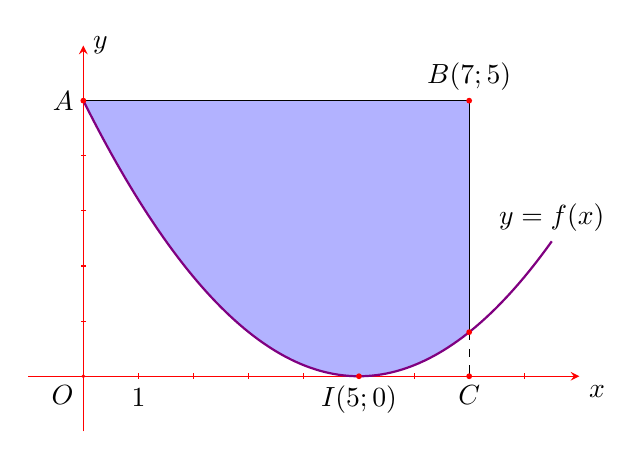
\begin{tikzpicture}[>=stealth, scale=.7]
			\fill[color=blue!30] (0,5) -- (7,5) -- (7,0.8) plot[domain=7:0] (\x, {0.2*(\x-5)^2}) -- cycle;
			\draw[->, red] (-1,0) -- (9,0) node[below right, black] {$x$};
			\draw[->, red] (0,-1) -- (0,6) node[right, black] {$y$};
			\node[below left] at (0,0) {$O$};
			\fill[red] (0,0) circle (1pt);
			\draw[red] (1,0.05) -- (1,-0.05) node[below, black] {$1$};
			\foreach \x in {2,3,4,6,8} \draw[red] (\x,0.05) -- (\x,-0.05);
			\foreach \y in {1,2,3,4} \draw[red] (0.05,\y) -- (-0.05,\y);
			\draw[thick, violet, domain=0:8.5, samples=100] plot (\x, {0.2*(\x-5)^2}) node[above, black] {$y=f(x)$};
			\draw (0,5) -- (7,5);
			\draw (7,5) -- (7,0.8);
			\draw[dashed] (7,0.8) -- (7,0) node[below] {$C$};
			\fill[red] (0,5) circle (1.5pt) node[left, black] {$A$};
			\fill[red] (7,5) circle (1.5pt) node[above, black] {$B(7;5)$};
			\fill[red] (5,0) circle (1.5pt) node[below, black] {$I(5;0)$};
			\fill[red] (7,0.8) circle (1.5pt);
			\fill[red] (7,0) circle (1.5pt);
		\end{tikzpicture}
	\end{center}
	\shortans{$26{,}1$}
	\loigiai{
		Parabol có dạng $(P)\colon y=f(x)=ax^2+bx+c$ (với $a \ne 0$).\\
		Dựa vào hình vẽ, $(P)$ đi qua điểm $A(0;5)$ và đỉnh $I$ của parabol có toạ độ $I(5;0)$.\\
		Suy ra ta có hệ phương trình
		\[\heva{&f(0)=5 \\ &f(5)=0 \\ &x_I = -\dfrac{b}{2a}=5} \Rightarrow \heva{&c=5 \\ &25a+5b+5=0 \\ &10a+b=0} \Rightarrow \heva{&a=\dfrac{1}{5} \\ &b=-2 \\ &c=5.}\]
		Suy ra phương trình parabol là $y=f(x)=\dfrac{1}{5}x^2-2x+5$.\\
		Diện tích của bảng quảng cáo (phần tô màu) là phần giới hạn bởi đường thẳng $y=5$ (cạnh $AB$) và đường parabol $(P)$ trên đoạn $[0;7]$ là
		\[S = \displaystyle\int\limits_0^7 \left| 5 - \left(\dfrac{1}{5}x^2-2x+5\right) \right| \mathrm{\,d}x = \displaystyle\int\limits_0^7 \left| -\dfrac{1}{5}x^2+2x \right| \mathrm{\,d}x = \dfrac{392}{15} \approx 26{,}1 \left(\text{m}^2\right).\]
	}
\end{ex}

%%==========Câu 2
\begin{ex}%[39-26-2-DaNang-SoGD-L1]%[Tuấn Anh,26-2-DuAnDeTHPT2025-2026]%[2D6H1-4]
Một giải đấu eSports có $8$ đội tuyển tham gia thi đấu loại trực tiếp, bắt đầu từ Tứ kết ($8$ đội được chia thành $4$ cặp, đội thắng trong mỗi cặp sẽ tiến vào Bán kết, đội thua bị loại). Ban Tổ chức đánh số hạt giống các đội theo thứ tự từ mạnh đến yếu là $1$ đến $8$. Việc bốc thăm chia $4$ cặp đấu Tứ kết được thực hiện ngẫu nhiên. Biết rằng khi thi đấu, đội có số hạt giống nhỏ hơn sẽ đánh bại đội có số hạt giống lớn hơn, tuy nhiên, có hai ngoại lệ: Đội số $8$ luôn đánh bại Đội số $1$ và Đội số $7$ luôn đánh bại Đội số $2$. Tính xác suất để Đội hạt giống số $3$ giành chức vô địch giải đấu (kết quả làm tròn đến hàng phần trăm).
\shortans{$0{,}03$}
\loigiai{
	Số phần tử của không gian mẫu (số cách xếp ngẫu nhiên $8$ đội vào $8$ vị trí của $4$ cặp đấu Tứ kết) là $n(\Omega) = 8!$.\\
	Gọi $A$ là biến cố: \lq\lq Đội hạt giống số $3$ giành chức vô địch giải đấu\rq\rq.\\
	Để Đội số $3$ vô địch thì Đội số $1$ và Đội số $2$ bắt buộc phải bị loại. Do Đội số $1$ chỉ có thể thua Đội số $8$ và Đội số $2$ chỉ có thể thua Đội số $7$ (theo ngoại lệ), nên ta cần xếp cặp cho các đội này đụng nhau ngay từ đầu để loại Đội $1$ và Đội $2$.\\
	Ta thực hiện việc xếp cặp như sau
	\begin{itemize}
		\item Công đoạn 1: Xếp Đội hạt giống $1$ gặp Đội hạt giống $8$ (để loại Đội $1$). Có $C_4^1 \cdot 2! = 8$ cách.
		\item Công đoạn 2: Xếp Đội hạt giống $2$ gặp Đội hạt giống $7$ (để loại Đội $2$). Có $C_3^1 \cdot 2! = 6$ cách.
		\item Công đoạn 3: $4$ đội còn lại (trong đó có Đội số $3$) được xếp ngẫu nhiên vào $4$ vị trí trống còn lại, có $4! = 24$ cách.
	\end{itemize}
	Suy ra số kết quả thuận lợi cho biến cố $A$ là $n(A) = 8 \cdot 6 \cdot 24 = 1152$ cách.\\
	Xác suất cần tìm là $P(A) = \dfrac{n(A)}{n(\Omega)} = \dfrac{1152}{8!} = \dfrac{1}{35} \approx 0{,}0285 \approx 0{,}03$.
}
\end{ex}

%%==========Câu 3
\begin{ex}%[39-26-2-DaNang-SoGD-L1]%[Tuấn Anh,26-2-DuAnDeTHPT2025-2026]%[0D2H2-3]
Trong một xưởng in, người ta sản xuất hai loại poster quảng bá sự kiện. Loại I sử dụng $2$ tờ giấy khổ lớn và $1$ đơn vị mực màu, thu được $35$ nghìn đồng. Loại II sử dụng $3$ tờ giấy khổ lớn và $2$ đơn vị mực màu, thu được $60$ nghìn đồng. Biết rằng xưởng chỉ có tối đa $210$ tờ giấy khổ lớn và $130$ đơn vị mực màu và mỗi poster phải được in trọn vẹn. Hỏi số tiền lớn nhất mà xưởng có thể thu được là bao nhiêu (nghìn đồng)?
\shortans{$4050$}
\loigiai{
	Gọi $x$, $y$ lần lượt là số poster loại I và số poster loại II ($x$, $y \geq 0$).\\
	Khi đó tổng số tờ giấy khổ lớn là $2x + 3y$; tổng số đơn vị mực màu là $x + 2y$.\\
	Bài toán đưa về tìm $x, y$ là nghiệm của hệ bất phương trình:
	$$ \heva{&2x + 3y \le 210 \\ &x + 2y \le 130 \\ &x \ge 0 \\ &y \ge 0} $$
	sao cho $P(x,y) = 35x + 60y$ có giá trị lớn nhất.\\
	Miền nghiệm của hệ bất phương trình là miền tứ giác $OABC$ với các đỉnh $O(0;0)$, $A(0;65)$, $B(30;50)$ và $C(105;0)$.\\
	Biểu thức $P(x,y) = 35x + 60y$ đạt giá trị lớn nhất tại một trong các đỉnh này:
	\begin{itemize}
		\item $P_O = 35 \cdot 0 + 60 \cdot 0 = 0$.
		\item $P_A = 35 \cdot 0 + 60 \cdot 65 = 3\,900$.
		\item $P_B = 35 \cdot 30 + 60 \cdot 50 = 4\,050$.
		\item $P_C = 35 \cdot 105 + 60 \cdot 0 = 3\,675$.
	\end{itemize}
	Vậy số tiền lớn nhất mà xưởng có thể thu được là $4\,050$ nghìn đồng (khi sản xuất $30$ poster loại I và $50$ poster loại II).
}
\end{ex}

%%==========Câu 4
\begin{ex}%[39-26-2-DaNang-SoGD-L1]%[Tuấn Anh,26-2-DuAnDeTHPT2025-2026]%[1H8H5-4]
Cho khối lăng trụ đứng $ABC.A'B'C'$ có độ dài cạnh bên bằng $4\sqrt{2}$ và đáy là tam giác $ABC$ vuông cân tại $C$, có $AC=4$. Gọi $M$ là trung điểm của cạnh $AA'$, tính khoảng cách giữa hai đường thẳng $CM$ và $AB$ (không làm tròn ở các bước trung gian).
\shortans{$2$}
\loigiai{
	\begin{center}
		\begin{tikzpicture}[line join=round,line cap=round,>=stealth,font=\footnotesize,scale=1,samples=300]
			\def\a{4}
			\def\h{4.5}
			\path 	(0:0) coordinate (A)
					++(0:\a) coordinate (C)
					++(-160:3*\a/4) coordinate (B)
					($(A)+(90:\h)$) coordinate (A')
					($(B)+(90:\h)$) coordinate (B')
					($(C)+(90:\h)$) coordinate (C')
					($(A)!0.5!(A')$) coordinate (M)
					($(C)!0.5!(C')$) coordinate (N)
					($(A)!0.5!(B)$) coordinate (P)
					($(N)!(C)!(P)$) coordinate (Q)
					;
			\draw[dashed] (A)--(C) (C')--(M) (A)--(N)--(P)--(C)--(Q);
			\draw (C)--(C') (B)--(B') (A)--(A') (A)--(B)--(C) (A')--(B')--(C')--cycle (N)--(B);
			\foreach \x/\g in {A/180,B/-45,C/0,A'/180,B'/-45,C'/0,M/180,N/0,P/200,Q/160} \fill (\x) circle (1pt) ($(\g:3.5mm)+(\x)$) node {$\x$};
			\foreach \x/\y/\z in {P/Q/C,B/P/C}{\draw pic[draw, angle radius=2mm]{right angle=\x--\y--\z};}
		\end{tikzpicture}
	\end{center}
	Gọi $N$ là trung điểm $CC'$. Dễ thấy $C'M \parallel AN \Rightarrow C'M \parallel (ABN)$.\\
	Do đó, khoảng cách cần tìm (do tính chất đối xứng $\mathrm{d}(CM, AB)=\mathrm{d}\left(C'M, AB\right)$) có thể được tính thông qua $C'M$\\
	\[\mathrm{d}\left(C'M,AB\right)=\mathrm{d}\left(C'M,(ABN)\right)=\mathrm{d}\left(C',(ABN)\right).\]
	Mà $CN = C'N$ nên $d(C', (ABN)) = d(C, (ABN))$.\\
	Kẻ $CP \perp AB$ và $CQ \perp NP$. Khi đó:
	$$ \heva{&CP \perp AB \\ &CN \perp AB} \Rightarrow AB \perp (CNP) \Rightarrow AB \perp CQ $$
	Suy ra $\heva{&CQ \perp NP \\ &CQ \perp AB} \Rightarrow CQ \perp (ABN) \Rightarrow d(C, (ABN)) = CQ$.\\
	Lại có $\dfrac{1}{CQ^2} = \dfrac{1}{CP^2} + \dfrac{1}{CN^2} = \dfrac{1}{AC^2} + \dfrac{1}{BC^2} + \dfrac{1}{CN^2}$.\\
	Biết $AC = BC = 4$; $CN = \dfrac{CC'}{2} = \dfrac{4\sqrt{2}}{2} = 2\sqrt{2}$.\\
	Thay số vào ta được \[\dfrac{1}{CQ^2} = \dfrac{1}{4^2} + \dfrac{1}{4^2} + \dfrac{1}{(2\sqrt{2})^2} = \dfrac{1}{16} + \dfrac{1}{16} + \dfrac{1}{8} = \dfrac{1}{4} \Rightarrow CQ = 2.\]
	Vậy khoảng cách cần tìm là $2$.
}
\end{ex}

%%==========Câu 5
\begin{ex}%[39-26-2-DaNang-SoGD-L1]%[Tuấn Anh,26-2-DuAnDeTHPT2025-2026]%[2D1H3-6]
Trong ngành hàng hải, lượng nhiên liệu tiêu thụ của một con tàu trong một đơn vị thời gian xấp xỉ tỷ lệ thuận với lập phương vận tốc của nó. Một tàu chở hàng xuất phát từ cảng Singapore đi đến cảng Tiên Sa cách $1\,000$ hải lý. Gọi $v$ (hải lý/giờ) là vận tốc của tàu ($v>0$). Dữ liệu kỹ thuật cho thấy chi phí nhiên liệu vận hành của con tàu là $0{,}02v^3$ (USD/giờ). Các chi phí vận hành cố định khác như lương thuyền viên, khấu hao, bảo hiểm,$\ldots$ không phụ thuộc vào vận tốc tàu là $625$ USD/giờ. Hỏi thuyền trưởng cần duy trì vận tốc trung bình là bao nhiêu hải lý/giờ để tổng chi phí cho toàn bộ chuyến đi là thấp nhất?
\shortans{$25$}
\loigiai{
	Thời gian để tàu đi hết quãng đường $1\,000$ hải lý là $t=\dfrac{1\,000}{v}$ (giờ).\\
	Tổng chi phí cho toàn bộ chuyến đi là
	\[C(v)=\left(0{,}02v^3+625\right)\cdot t=\left(0{,}02v^3+625\right)\cdot \dfrac{1\,000}{v}=20v^2+\dfrac{625\,000}{v}.\]
	Ta có $C'(v)=40v-\dfrac{625\,000}{v^2}$.\\
	Ta lại có $C'(v)=0\Leftrightarrow 40v = \dfrac{625\,000}{v^2} \Leftrightarrow v^3=15\,625\Leftrightarrow v=25$.\\
	Bảng biến thiên
	\begin{center}
		
\begin{tikzpicture}
			\tkzTabInit[lgt=1.2,espcl=3]
			{$x$ /1.2, $C’(x)$ /1.2, $C(x)$ /2.5}
			{$0$,$25$,$+\infty$}
			\tkzTabLine{,-,z,+,}
			\tkzTabVar{+/$+\infty$,-/$37\,500$,+/$+\infty$}
		\end{tikzpicture}
	\end{center}
	Suy ra hàm số $C(v)$ đạt giá trị nhỏ nhất tại $v=25$.\\
	Vậy thuyền trưởng cần duy trì vận tốc tối ưu là $25$ hải lý/giờ để chi phí thấp nhất.
}
\end{ex}

%%==========Câu 6
\begin{ex}%[39-26-2-DaNang-SoGD-L1]%[Tuấn Anh,26-2-DuAnDeTHPT2025-2026]%[2D4V3-1]
Cho hàm số $f(x)=2^{x^2}$ và hàm số $g(x)=\sqrt{\log_2 x}$. Giả sử $S=\displaystyle\int\limits_1^{20}f(x)\mathrm{\,d}x+\displaystyle\int\limits_2^{2^{400}}g(x)\mathrm{\,d}x$ được viết dưới dạng $S=a\cdot 2^b-c$, với $b$ là số nguyên và $a, c$ là các số nguyên tố. Tính $a+b+c$.
\shortans{$409$}
\loigiai{
	Xét hàm số $y=f(x)=2^{x^2}$ trên đoạn $[1; 20]$.\\
	Thực hiện phép đối xứng qua đường phân giác $d\colon y=x$ thay $x$ bởi $y$ và $y$ bởi $x$ vào phương trình $y=2^{x^2}$ (với $x,y > 0$), ta được
	\[x = 2^{y^2} \Leftrightarrow y^2 = \log_2 x \Leftrightarrow y = \sqrt{\log_2 x} = g(x).\]
	Suy ra đồ thị của hai hàm số $y=f(x)$ và $y=g(x)$ đối xứng nhau qua đường thẳng $d\colon y=x$.\\
	Lại có $f(1)=2$, $f(20)=2^{400}$ nên tương ứng đối với hàm ngược $g(2)=1$, $g\left(2^{400}\right)=20$.\\
	Dựa vào tính chất đối xứng, ta có
	\begin{itemize}
		\item $\displaystyle\int\limits_1^{20} f(x) \mathrm{\,d}x$ chính là diện tích $S_1$ nằm dưới đồ thị $f(x)$.
		\item $\displaystyle\int\limits_2^{2^{400}} g(x) \mathrm{\,d}x$ chính là diện tích $S_2$ nằm dưới đồ thị $g(x)$, đồng thời cũng tương đương với phần diện tích được giới hạn bởi trục $Oy$, đồ thị $f(x)$ và hai đường thẳng $y=2, y=2^{400}$.
	\end{itemize}
	Do đó, tổng của hai tích phân này bằng diện tích của hình chữ nhật lớn tạo bởi các đỉnh $(0;0)$, $(20;0)$, $\left(20;2^{400}\right)$, $\left(0;2^{400}\right)$ trừ đi diện tích hình chữ nhật nhỏ tạo bởi $(0;0)$, $(1;0)$, $(1;2)$, $(0;2)$.\\
	Cụ thể
	\[S = \displaystyle\int\limits_1^{20} f(x) \mathrm{\,d}x + \displaystyle\int\limits_2^{2^{400}} g(x) \mathrm{\,d}x = 20 \cdot 2^{400} - 1 \cdot 2 = 5 \cdot 2^{402} - 2.\]
	Theo giả thiết $S = a \cdot 2^b - c$, ta đồng nhất hệ số thu được $a=5$, $b=402$, $c=2$ (thỏa mãn $a, c$ là số nguyên tố).\\
	Vậy $a+b+c = 5 + 402 + 2 = 409$.
}
\end{ex}

\Closesolutionfile{ans}

\indapan{6}{ans/ans-39-26-2-DaNang-SoGD-L1-LC}
\indapan{4}{ans/ans-39-26-2-DaNang-SoGD-L1-DS}
\indapan{6}{ans/ans-39-26-2-DaNang-SoGD-L1-KQ}
